\chapter{Wheeler Graphs}

\section{Definition of Wheeler Graph}

\begin{definition} \label{def_wheeler_graphs}
    A Wheeler graph $G=(V,E)$ is defined as a directed graph with labeled edges, equipped with a total order $<_{\pi}$ on the nodes in $V$, which satisfies the following three axioms:

    \begin{enumerate}[(i)]
        \item All vertices with in-degree $0$ must precede those with a greater in-degree in the ordering; \label{axiom_1}
    \suspend{enumerate}
    For every pair of edges $(u_1,v_1,k_1)$ and $(u_2,v_2,k_2)$:
    \resume{enumerate}[{[(i)]}]
        \item $k_1<k_2 \Rightarrow v_1<_{\pi}v_2$; \label{axiom_2}
        \item $(k_1=k_2) \wedge (u_1<_{\pi}u_2) \Rightarrow v_1\leq_{\pi}v_2$. \label{axiom_3}
    \end{enumerate}
\end{definition}

\section{Examples of Wheeler Graphs}
\begin{figure}[H]
    \centering
    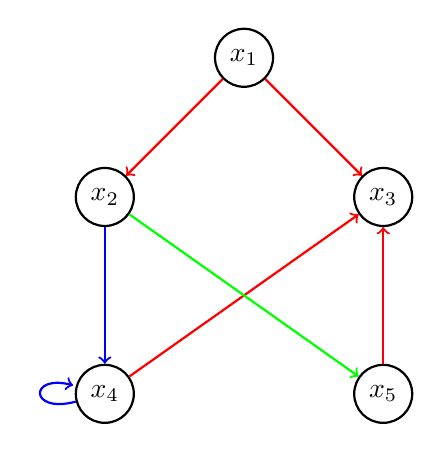
\begin{tikzpicture}[node distance={25mm}, thick, auto=center, main/.style = {draw, circle}]
        \node[main] (1) {$x_1$};
        \node[main] (2) [below left of=1] {$x_2$};
        \node[main] (3) [below right of=1] {$x_3$};
        \node[main] (4) [below of=2] {$x_4$};
        \node[main] (5) [below of=3]{$x_5$};
        \draw[red, ->] (1) -- (3);
        \draw[red, ->] (1) -- (2);
        \draw[red, ->] (4) -- (3);
        \draw[red, ->] (5) -- (3);
        \draw[green, ->] (2) -- (5);
        \draw[blue, ->] (2) -- (4);
        \draw (4) edge[blue, loop left] (4);
    \end{tikzpicture}
    \caption[Example of a Wheeler Graph]{Example of a Wheeler graph with $\sigma=3$. The label order is as follows: red $<$ blue $<$ green. The resulting total order of nodes is: $x_1<x_2<x_3<x_4<x_5$.}
    \label{fig:wheeler_example}
\end{figure}

Consider Figure \ref{fig:wheeler_example}. Axiom (\ref{axiom_1}) states that nodes with no incoming edges (in-degree $0$) must be positioned at the beginning of the total order and never after nodes with a greater in-degree. In the example, node $x_1$ is the only node with in-degree $0$, so it is placed as the first element in the resulting total order.

\begin{figure}[H]
    \centering
    \begin{tabular}{cc}
        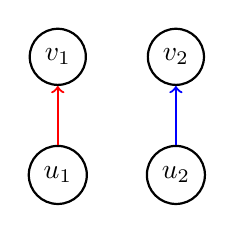
\begin{tikzpicture}[node distance={15mm}, thick, auto=center, main/.style = {draw, circle}]
            \node[main] (1)  {$u_1$};
            \node[main] (2) [right of=1] {$u_2$};
            \node[main] (3) [above of=1] {$v_1$};
            \node[main] (4) [above of=2] {$v_2$};
            \draw[->, red] (1) -- (3);
            \draw[->, blue] (2) -- (4);
        \end{tikzpicture} &
        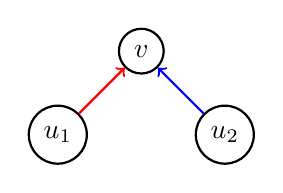
\begin{tikzpicture}[node distance={15mm}, thick, auto=center, main/.style = {draw, circle}]
            \node[main] (3) {$v$};
            \node[main] (1) [below left of=3] {$u_1$};
            \node[main] (2) [below right of=3] {$u_2$};
            \draw[->, red] (1) -- (3);
            \draw[->, blue] (2) -- (3);
        \end{tikzpicture} \\
        (a) & (b) \\
    \end{tabular}
    \caption{Examples for Axiom (\ref{axiom_2}).}
    \label{fig:example_axiom_2}
\end{figure}

To better understand Axiom (\ref{axiom_2}), consider Figure \ref{fig:example_axiom_2}. In example (a), we have two edges $(u_1,v_1,red)$ and $(u_2,v_2,blue)$ with $red<blue$. According to the axiom, since the edges have different labels, the destination node of the edge with the smaller label (in this case $v_1$) must precede the destination node of the edge with the larger label, so we obtain $v_1$ before $v_2$ in the total order.

In example (b), we instead have two edges $(u_1,v,red)$ and $(u_2,v,blue)$ with $red<blue$, but they share the same destination node. This case is not accepted by the second axiom because, if the labels are different, their order must be reflected in the destination nodes, which thus cannot be the same.

\begin{figure}[H]
    \centering
    \begin{tabular}{cc}
        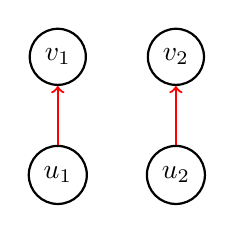
\begin{tikzpicture}[node distance={15mm}, thick, auto=center, main/.style = {draw, circle}]
            \node[main] (1)  {$u_1$};
            \node[main] (2) [right of=1] {$u_2$};
            \node[main] (3) [above of=1] {$v_1$};
            \node[main] (4) [above of=2] {$v_2$};
            \draw[->, red] (1) -- (3);
            \draw[->, red] (2) -- (4);
        \end{tikzpicture} &
        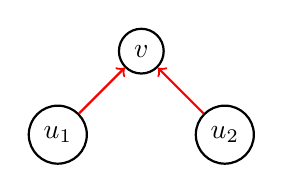
\begin{tikzpicture}[node distance={15mm}, thick, auto=center, main/.style = {draw, circle}]
            \node[main] (3) {$v$};
            \node[main] (1) [below left of=3] {$u_1$};
            \node[main] (2) [below right of=3] {$u_2$};
            \draw[->, red] (1) -- (3);
            \draw[->, red] (2) -- (3);
        \end{tikzpicture} \\
        (a) & (b) \\
    \end{tabular}
    \caption{Examples for Axiom (\ref{axiom_3}).}
    \label{fig:example_axiom_3}
\end{figure}

To better understand Axiom (\ref{axiom_3}), consider Figure \ref{fig:example_axiom_3}. In example (a), we have two edges $(u_1,v_1,red)$ and $(u_2,v_2,red)$ with $u_1<u_2$. The axiom applies here because the edges share the same label. Consequently, the order of the source nodes propagates to the destination nodes of the two edges. Specifically, the destination node of the edge whose source node is smaller in the total order must not be larger than the destination node of the edge whose source node is larger. In this case, since $u_1<u_2$, we obtain $v_1\leq v_2$.

In example (b), we consider the case where the two edges $(u_1,v,red)$ and $(u_2,v,red)$ with $u_1<u_2$ have the same label and share the same destination node. Again, the axiom applies, requiring that $v_1\leq v_2$. In this case, we obtain $v_1=v_2$.

\section{Properties of Wheeler Graphs}
The following is a list of some properties of Wheeler graphs that can be derived from the axioms (Definition \ref{def_wheeler_graphs}).

\begin{lemma} \label{property_1}
    All incoming edges to a node $v$ must have the same label. This property makes it equivalent to label either the nodes or the edges of the graph.
\end{lemma}

\begin{proof}
    Lemma \ref{property_1} is a natural derivation of the second Wheeler axiom (Definition \ref{def_wheeler_graphs}). It states that given two edges $(u_1,v_1,k_1)$ and $(u_2,v_2,k_2)$ with $k_1<k_2$, the order of the edge labels propagates to the destination nodes, implying $v_1<v_2$. This means that the destination nodes $v_1$ and $v_2$ cannot be the same if they receive incoming edges with different labels; otherwise, the considered graph would not be Wheeler.
\end{proof}

\begin{lemma} \label{property_2}
    A node $v$ may have multiple outgoing edges with the same label.
\end{lemma}

\begin{proof}
    Assume, for contradiction, that the statement does not hold and that a node $v$ cannot have multiple outgoing edges with the same label if the graph is Wheeler. The graph in Figure \ref{fig:wheeler_example} is a valid counterexample demonstrating the opposite, as node $x_1$ has two outgoing edges labeled $red$, and the graph is Wheeler. This leads to a contradiction.
\end{proof}

\begin{lemma} \label{property_3}
    Consider a Wheeler graph $G=(V,E)$ with labeling defined over a set $\Sigma=\{a,b,c\}$, where the label order is $a<b<c$. Let $V_a \subseteq V$ be the set of vertices with label $a$ (i.e., those with incoming edges labeled $a$), $V_b \subseteq V$ the set of vertices with label $b$, and $V_c \subseteq V$ the set of vertices with label $c$. Also, let $u_a \in V_a$, $u_b \in V_b$, and $u_c \in V_c$. Then, in the context of vertex ordering in the graph, it holds that $u_a < u_b < u_c$. More generally, all vertices in $V_k$ for a certain label $k$ will be consecutive in the ordering, with no nodes of other labels interspersed among them in the total order.
\end{lemma}

\begin{proof}
    Lemma \ref{property_3} follows naturally from the second Wheeler axiom (Definition \ref{def_wheeler_graphs}). Consider a Wheeler graph $G=(V,E)$ with labeling over a set $\Sigma=\{a,b\}$, where the order of labels is $a<b$. Let $V_a \subseteq V$ be the set of vertices labeled $a$ and $V_b \subseteq V$ be the set of vertices labeled $b$. Suppose, for contradiction, that there exist two nodes $u_a \in V_a$ and $u_b \in V_b$ such that $u_b < u_a$ in the Wheeler ordering.
    
    Since $u_a \in V_a$ and $u_b \in V_b$, by the definition of sets $V_a$ and $V_b$, there must exist two edges $(v_1, u_a, a)$ and $(v_2, u_b, b)$. However, this leads to a contradiction because the second axiom states that for two edges $(u_1,v_1,k_1)$ and $(u_2,v_2,k_2)$ with $k_1<k_2$, the order of edge labels must be reflected in the destination nodes, meaning $v_1<v_2$. In our case, $a<b$, but $u_b < u_a$, implying the graph is not Wheeler.
\end{proof}

\begin{lemma} \label{property_4}
    Consider a total Wheeler order. Let $V_k$ be the set containing all nodes with the same label $k$. Let $V_k^1$ and $V_k^2$ be two partitions of $V_k$, where $V_k^1$ contains all nodes $v_1$ with incoming edges from nodes preceding $v_1$ in the total order, while $V_k^2$ contains all nodes $v_2$ with incoming edges from nodes following $v_2$ in the total order. Consequently, the intersection of $V_k^1$ and $V_k^2$ contains at most one vertex $u$, and all vertices in $V_k^1 \setminus \{u\}$ precede those in $V_k^2$ in the ordering. Moreover, given a vertex $v \in V_k^1$, there cannot exist an edge $(v, z, k)$ with $z<v$, and similarly, given a vertex $v \in V_k^2$, there cannot exist an edge $(v, z, k)$ with $z>v$ (see \cite{15}).
\end{lemma}

\subsection{Path Coherence}
The following defines \textit{path coherence} and a related property of Wheeler graphs introduced and proven in \cite{1}.

\begin{definition}[Path Coherence]
    A labeled directed graph $G$ is said to be \textit{path coherent} if there exists a total order of nodes such that, for every consecutive interval $[i, j]$ of nodes and a string $\alpha$, the nodes reachable from those in $[i, j]$ in $|\alpha |$ steps, following edges whose labels form $\alpha$ when concatenated, themselves form an interval in the total order.
\end{definition}

\begin{lemma} \label{property_5}
    A Wheeler graph is path coherent with respect to any possible Wheeler order of the nodes.
\end{lemma}

Thanks to this crucial property, it was proven in \cite{1} that if the state diagram of a finite-state automaton is a Wheeler graph, then, due to Lemma \ref{property_5}, the nodes can be ordered so that for any string, the nodes reachable from the initial state(s) by processing that string are consecutive. This means that even if the automaton is non-deterministic, it can still be stored compactly and used to process strings efficiently.

\subsection{Topological Ordering for \texorpdfstring{$\sigma=1$}{Lg}}
The following defines \textit{topological ordering} and a related property of Wheeler graphs introduced and proven in \cite{15}.

\begin{definition}[Topological Ordering]
    A topological ordering is a linear ordering of all vertices of a directed graph. The nodes of a graph are said to be topologically ordered if they are arranged such that each node precedes all nodes connected to its outgoing edges. The topological ordering of a graph may not be unique. In the worst case, there can be $n!$ different topological orderings corresponding to all possible permutations of the $n$ nodes. A topological ordering is possible if and only if the graph has no directed cycles, meaning it is a directed acyclic graph (DAG) \cite{16}.
\end{definition}

\begin{lemma} \label{property_6}
    For $\sigma=1$, every Wheeler order also represents a topological ordering, except for vertices with self-loops, which must be placed at the end of the order since a cyclic graph cannot have a valid topological ordering.
\end{lemma}

This property follows from Lemma \ref{proprietà_4} and the first axiom (Definition \ref{def_wheeler_graphs}). Finally, it is important to highlight that this result is used in \cite{15} to prove that the Wheeler graph recognition problem can be solved in linear time when $\sigma=1$.

\begingroup
\sloppy
\raggedright
\section{Bipartite Representation of Wheeler Graphs} \label{rapp_bipartita}
\endgroup
The following section explains a simple and intuitive technique used to graphically check whether a directed labeled graph, along with its total node ordering, satisfies the three Wheeler axioms (Definition \ref{def_wheeler_graphs}). More specifically, the technique involves representing the graph as a bipartite graph with useful properties related to the three Wheeler axioms. Additionally, later in the text, we will see how this idea is also useful for the Wheelerization problem of a graph.

\subsection{Construction of the Bipartite Graph}
Consider a directed labeled graph on the edges $G=(V,E)$ where $V=\{x_1,\dots,x_n\}$ and a total ordering of $V$ (in the example, consider $x_1<x_2<\dots<x_n$). The bipartite graph (Section \ref{def_bipartito}) $B=(V_1,V_2,E_B)$ is constructed as follows:

\begin{itemize}
    \item $V_1=\{x_i^s : i \in [1, n]\}$. Where the node $x_i^s \in V_1$ corresponds to the node $x_i \in V$ for $1 < i < n$. This set is thus composed of the nodes in $V$, and is ordered according to the given ordering.
    \item $V_2=\{x_i^d : i \in [1, n]\}$. Where the node $x_i^d \in V_2$ corresponds to the node $x_i \in V$ for $1 < i < n$. This set is also composed of the nodes in $V$, and is ordered according to the given ordering.
    \item $E_B=\{(u, v) : u \in V_1 \wedge v \in V_2 \wedge (u,v) \in E\}$. Therefore, for every edge $(x_i,x_j) \in E$, a corresponding edge is created in the bipartite graph such that $x_i = x_i^s \in V_1$ and $x_j=x_j^d \in V_2$ with $i, j \in [1, n]$. For example, given the edge $(x_1, x_4)$, an edge is created between $x_1^s$ and $x_4^d$ (edge $(x_1^s,x_4^d)$ in the bipartite graph).
\end{itemize}

The following explanation assumes a vertical construction of the bipartite graph. As a result, since the nodes in $V_1$ and $V_2$ are ordered according to the total ordering of $V$ (in the example, we have $x_1^s<x_2^s<\dots<x_n^s$ and $x_1^d<x_2^d<\dots<x_n^d$), a node $x_i^s \in V_1$ is positioned graphically above a node $x_j^s \in V_1$ if and only if $i < j$ in the ordering, and similarly, a node $x_i^d \in V_2$ is positioned graphically above a node $x_j^d \in V_2$ if and only if $i < j$ in the ordering.

This vertical construction implies that the nodes in the set $V_1$ will be arranged in ascending order downward, maintaining the total ordering. Similarly, the nodes in the set $V_2$ will be arranged in ascending order downward, respecting the established ordering. In this way, the vertical position of the nodes reflects the ordering of the nodes within the graph. See the example in Figure \ref{fig:bipartite_example}-(a), which shows the bipartite representation of the graph in Figure \ref{fig:wheeler_example}.

\subsection{Properties of the Bipartite Graph}
As introduced earlier, the bipartite representation allows us to easily verify whether the three Wheeler axioms (Definition \ref{def_wheeler_graphs}) are satisfied by the graph $G$ and the ordering on $V$ (consider the graph and ordering defined in the previous section). The properties related to the axioms are as follows:
\begin{itemize}
    \item Axiom (\ref{axiom_1}) is satisfied if for every pair of nodes $u, v \in V$ it holds that if $indegree(u) = 0 \wedge indegree(v) > 0$, then $u < v$ in the ordering.
    \item Axiom (\ref{axiom_2}) is satisfied if every node in the bipartite graph has all incoming edges with the same label, and moreover, the order of the labels respects the node ordering. Formally, let $\lambda(u)$ be a function that returns the label of a given node $u \in V$. It must hold that $\lambda(x_1) \leq \lambda(x_2) \leq \dots \leq \lambda(x_n)$.
    \item Axiom (\ref{axiom_3}) is satisfied if there are no edges with the same label crossing in the bipartite graph. Formally, a crossing is defined as follows: let $(x_i^s,x_j^d,k_1)$, $(x_k^s,x_w^d,k_2)$ be two edges of the bipartite graph labeled $k_1$ and $k_2$, respectively, a crossing occurs if $(i < k \wedge j > w) \lor (i > k \wedge j < w)$, where the subscripts of the nodes indicate their position in the ordering.
\end{itemize}

\begingroup
\sloppy
\raggedright
\subsection{Examples of Bipartite Representation of Wheeler Graphs}
\endgroup
Consider the Wheeler graph shown in Figure \ref{fig:wheeler_example}, and the resulting bipartite graph shown in Figure \ref{fig:bipartite_example}-(a). 

\begin{figure}[H]
    \centering
    \begin{tabular}{cc}
        \begin{tikzpicture}[node distance={15mm}, thick, auto=center, main/.style = {draw, circle}] 
            \node[main] (1s) {$x_1^s$};
            \node[main] (2s) [below of=1s] {$x_2^s$}; 
            \node[main] (3s) [below of=2s] {$x_3^s$};
            \node[main] (4s) [below of=3s] {$x_4^s$};
            \node[main] (5s) [below of=4s] {$x_5^s$};
            \node[main] (1d) [right=2cm of 1s] {$x_1^d$};
            \node[main] (2d) [below of=1d] {$x_2^d$}; 
            \node[main] (3d) [below of=2d] {$x_3^d$};
            \node[main] (4d) [below of=3d] {$x_4^d$};
            \node[main] (5d) [below of=4d] {$x_5^d$};
            \draw[red, ->] (1s) -- (3d);
            \draw[red, ->] (1s) -- (2d);
            \draw[red, ->] (4s) -- (3d);
            \draw[red, ->] (5s) -- (3d);
            \draw[green, ->] (2s) -- (5d);
            \draw[blue, ->] (2s) -- (4d);
            \draw[blue, ->] (4s) -- (4d);
        \end{tikzpicture} &
        \begin{tikzpicture}[node distance={15mm}, thick, auto=center, main/.style = {draw, circle}] 
            \node[main] (3s) {$x_3^s$};
            \node[main] (2s) [below of=3s] {$x_2^s$}; 
            \node[main] (1s) [below of=2s] {$x_1^s$};
            \node[main] (4s) [below of=1s] {$x_4^s$};
            \node[main] (5s) [below of=4s] {$x_5^s$};
            \node[main] (3d) [right=2cm of 3s] {$x_3^d$};
            \node[main] (2d) [below of=3d] {$x_2^d$}; 
            \node[main] (1d) [below of=2d] {$x_1^d$};
            \node[main] (4d) [below of=1d] {$x_4^d$};
            \node[main] (5d) [below of=4d] {$x_5^d$};
            \draw[red, ->] (1s) -- (3d);
            \draw[red, ->] (1s) -- (2d);
            \draw[red, ->] (4s) -- (3d);
            \draw[red, ->] (5s) -- (3d);
            \draw[green, ->] (2s) -- (5d);
            \draw[blue, ->] (2s) -- (4d);
            \draw[blue, ->] (4s) -- (4d);
        \end{tikzpicture} \\
        (a) & (b) \\
    \end{tabular}
    \caption[Bipartite Representation of a Wheeler Graph]{Example of bipartite representation of the graph in Figure \ref{fig:wheeler_example}, useful for verifying that it satisfies the three Wheeler axioms. (a) respects the correct ordering, while (b) does not.}
    \label{fig:bipartite_example}
\end{figure}

As we can observe, the three axioms are satisfied, because:
\begin{itemize}
    \item $x_1$ is the only node with in-degree $0$ and is at the beginning of the ordering;
    \item all nodes have all incoming edges with the same label\footnote{In the image, the colors represent the labels.};
    \item starting from the top, the sequence of labels assigned to the incoming edges on each node is as follows: red, red, blue, green, which respects the ordering of the alphabet considered (red $<$ blue $<$ green);
    \item there are no crossings between edges with the same color in the bipartite graph.
\end{itemize}
Therefore, we can confidently assert that the graph in question is a Wheeler graph for the given node order.

The example in Figure \ref{fig:bipartite_example}-(b), however, is constructed using the graph from Figure \ref{fig:wheeler_example}, but considering the following node order: $x_3<x_2<x_1<x_4<x_5$. The resulting bipartite graph shows that the graph from Figure \ref{fig:wheeler_example} with the order $x_3<x_2<x_1<x_4<x_5$ is not a Wheeler graph, because:
\begin{itemize}
    \item the first axiom is not satisfied since node $x_1$ is not at the beginning of the ordering;
    \item the third axiom is not satisfied because there are red edges that cross in the bipartite graph.
\end{itemize}